\documentclass{beamer}
\usetheme{metropolis} % Use metropolis theme

\renewcommand{\footnoterule}{%
  \hspace{10cm}
  \kern -3pt
  \hrule width \textwidth height 1pt
  \kern 2pt
}
\usepackage[utf8]{inputenc}
\usepackage[T1]{fontenc}
\usepackage[british]{babel}
\usepackage[autostyle, english = british]{csquotes}
\usepackage[%
  backend=biber,
  doi=false,
  url=false,
  isbn=false,
  eprint=false,
  style=authoryear,
  hyperref=true,
  maxnames=2,
  minnames=1,
  maxbibnames=99,
  firstinits,
  uniquename=init]{biblatex}
\addbibresource{../bibliography.bib}

\usepackage{caption}
\usepackage{xpatch}
\usepackage{bm}
\usepackage{amsmath}
\usepackage{mathtools} % for \mathclap
\usepackage{varioref}
\usepackage{siunitx}
\usepackage{hyperref}
\usepackage[noabbrev]{cleveref}
\newcommand{\creflastconjunction}{, and\nobreakspace} % use Oxford comma
\usepackage{todonotes}
\usepackage{phaistos}
\usepackage{multimedia}
\usepackage{tikz}
\usetikzlibrary{arrows, positioning, shapes.geometric}
\usetikzlibrary{calc}
\usepackage{pgfgantt}


\graphicspath{{../../figures/}}

\newcommand{\cn}{\textbf{TODO: Citation}}

\title{Data-Driven Models for Zebrafish Motion}
\author{Lukas Krenz}
\date{April 05, 2018} 
\institute{TUM, Chair for Computer Aided Medical Procedures \textit{\&} Augmented Reality\\
Interdisciplinary Project}

\begin{document}
\maketitle
\begin{frame}{Introduction}
Advisers: Dr.\ Jacob Davidson (Couzin Lab), Nicola Rieke (CAMP)

Supervisor: Prof.\ Dr.\ Nassir Navab (CAMP)

Idea:
\begin{itemize}
\item Compare three \textbf{increasingly complex} data-driven models for motion of juvenile zebrafish
\item Investigate pair-wise motion but create flexible models that extend to larger groups
\item Model should capture motion of fish observed in experiments with \textbf{real fish}
\end{itemize}

\end{frame}

% \begin{frame}{Zebrafish: Burst-and-coast Motion} 
%     \begin{figure}[H]
%     \centering
%     \movie[width=0.66\textwidth, height=0.66\textwidth, autostart,, loop, poster]{}{motion_experiment.mp4}
%     \caption*{Example of zebrafish motion}
%     \label{fig:calovi-sim}
%   \end{figure}
% \end{frame}

\begin{frame}
  \frametitle{Modelling Fish Motion}
Data: Roughly \textbf{100k kicks} from 10 experiments with 2 fish swimming, each for 1h

Segmentation into kicks as pre-processing step

Model \textbf{for each} fish: Map wall distance/angle and neighbour distance/angle to heading change $\delta \phi$, or to kick trajectory
\begin{columns}
  \begin{column}{0.24\linewidth}
    \begin{figure}[h]
      \centering
    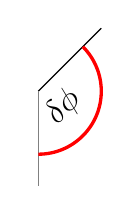
\begin{tikzpicture}[scale=0.4]
   \draw[] (3, 3)--(5,5); % our fish at t
   \node[rotate=45] at (4.5,4.5) {\textcolor{red}\PHtunny}; % head
   
   \draw[gray] (3.0, 0)--(3.0, 3.0); % fish at t - 1
   \node[rotate=90] at (3.0,2.5) {\textcolor{gray}\PHtunny}; % fish at t -1

   \draw [red,very thick] (3.0, 1.0) arc (-90:45:2);
   \node[rotate=45] at (3.8, 2.5) {\large$\delta\phi$};
 \end{tikzpicture} 
 \caption*{Heading change}
\end{figure}
\end{column}

\begin{column}{0.4\linewidth}
  \begin{figure}[h]
    \centering
\includegraphics[clip, width=0.8\linewidth]{kick_duration.pdf}
    \caption*{Kick duration}
  \end{figure}
\end{column}

\begin{column}{0.4\linewidth}
  \begin{figure}[h]
    \centering
\includegraphics[clip, width=0.8\linewidth]{kick_length.pdf}
    \caption*{Kick length}
  \end{figure}
\end{column}

\end{columns}
\end{frame}

\begin{frame}{First Model: Force Based (Calovi et al\footnote{\hspace*{0.1cm}\textit{Disentangling and modeling interactions in fish with burst-and-coast swimming}, arXiv, 2017, Calovi, D.S., Litchinko, A., Lecheval, V., Lopez, U., Escudero, A.P., Chaté, H., Sire, C. and Theraulaz, G.})}
\begin{enumerate}
\item Discrete model, model heading change $\delta \phi$ for kicks
\item Decision process only uses \textbf{current status}
\item \textbf{Explicit} alignment and attraction term
\item Each term split into product of exponential decay and Fourier sums
\item Hard to fit - \textbf{not} convex
\end{enumerate}
Full model:
\begin{align*}
  \label{eq:calovi-model}
  \delta \phi = \text{noise} + \text{wall avoidance} + \text{attraction} + \text{alignment}
\end{align*}
\end{frame}

\begin{frame}
  \frametitle{Calovi - (Preliminary) Wall Fit}
 \begin{columns}
   \begin{column}{0.5\textwidth}
     \begin{figure}[h]
       \centering
\includegraphics[clip, width=1\linewidth]{wall_force.pdf}
       \caption*{$f(r_w)$}
     \end{figure}
   \end{column}
   
   \begin{column}{0.5\textwidth}
     \begin{figure}[h]
       \centering
\includegraphics[clip, width=1\linewidth]{wall_odd.pdf}
       \caption*{$O(\theta_w)$}
     \end{figure}
   \end{column}
\end{columns}
Limit dataset to kicks with neglible wall force (using $f(r_w)$)
\end{frame}

\begin{frame}
  \frametitle{Second model: Spatio-Temporal Receptive Field}
 \begin{columns}
   \begin{column}{0.5\textwidth}
  \begin{tikzpicture}[scale=0.5]
   %\draw[red] (3, 3)--(5,5);
   \draw[ultra thick] (0,0)--(0,5);
   %\draw (4,-3)--(4,3);
   \node[rotate=45] at (4.5,4.5) {\textcolor{red}\PHtunny};
   \node[rotate=90] at (2.5,2.5) {\PHtunny};
   \node[rotate=90] at (2.5,0.5) {\textcolor{white}\PHtunny}; % quick hack to align stuff
 \end{tikzpicture}

 \textbf{No memory}: Only current position, etc.
\end{column}~\begin{column}{0.5\textwidth}
  \begin{tikzpicture}[scale=0.5]
   \draw[red] (3, 3)--(5,5); % our fish
   \draw[ultra thick] (0,0)--(0,5); % wall
   \draw[gray] (2.5, 0)--(2.5,2.5);
   \node[rotate=45] at (4.5,4.5) {\textcolor{red}\PHtunny};
   \node[rotate=90] at (2.5,2.5) {\PHtunny};
   \node[rotate=90] at (2.5,0.5) {\textcolor{gray}\PHtunny};
 \end{tikzpicture}

 \textbf{Memory}: Current position and trace
   \end{column}
 \end{columns}
  Drop assumption of irrelevant past

  Approximate reaction to social forces by \textbf{weighted sum} over past environment influences (e.g.\ distances, angles)

  Linear model with memory

  Extends easily to larger fish groups, thanks to binning
  (dividing space around fish into sub-areas)
\end{frame}

\begin{frame}{Bins}
 \begin{columns}
   \begin{column}{0.5\textwidth}
     \begin{figure}[h]
       \centering
\includegraphics[clip, width=1\linewidth, draft]{wall_force.pdf}
       \caption*{Regular Bins}
     \end{figure}
   \end{column}
   
   \begin{column}{0.5\textwidth}
     \begin{figure}[h]
       \centering
\includegraphics[clip, width=1\linewidth, draft]{wall_odd.pdf}
       \caption*{Adaptive Bins}
     \end{figure}
   \end{column}
  \end{columns}

Color indicates linear model coefficients (position only)

Over time: Weighted sum over past before kick. Two options:
\begin{enumerate}
\item keep spatial bins constant  
\item one set of coefficients per time step
\end{enumerate}
\end{frame}

\begin{frame}
  \frametitle{Third Model: Neural Network}
  Some evidence\footnote{\textit{Inferring the structure and dynamics of interactions in schooling fish}, Proceedings of the National Academy of Sciences, 2011, Katz, Y., Tunstrøm, K., Ioannou, C. C., Huepe, C., and Couzin, I. D.} for non-linear effects in collective animal motion

  Idea: Approximate reaction to social influences with a neural network

  Time series data, strong autocorrelation

  Use models such as \textbf{recurrent neural networks} (e.g.\ LSTM, GRU) or model convolution over past directly (e.g.\ with neural networks with causal convolutions)
  
  \textbf{Highly} non-linear \textbf{black-box} model with memory
\end{frame}

\end{document}